\documentclass[draftclsnofoot,onecolumn]{IEEEtran}

\usepackage{amsmath,amsthm,amssymb}
\usepackage{graphicx}
\graphicspath{{/home/jingle/figures/}} %path to graphs
\usepackage{subfigure}

\usepackage{url}
\usepackage{cite}

% correct bad hyphenation here
\hyphenation{op-tical net-works semi-conduc-tor}

\begin{document}

\title{Traf: A Camera Based System for Traffic Flow Analysis}
\maketitle
\author{fsb}

\begin{abstract}

In this paper, we present a camera based system(Traf) to count automotive vehicles for traffic flow analysis use. The system employs the method of background subtraction by comparing differences between foreground and background. The background model is initialed by averaging first 50 frames, and adapted to environment change by introducing an adapting parameter $\lambda$. Compared to state-of-art method, it is more robust, adaptive and economical.

\end{abstract}


%--------------------------------------------------------------------------------
% what and why ?
\section{Introduction}
%近年来,随着我国经济的发展,综合国力的不断提升,机动车保有量迅速增加,导致交通拥堵现象非常严重。交通管理的成本也越来越高,有效采集交通参数,合理分配道路资源是解决这些问题的关键。基于视频图像的车流量检测是采集交通参数的方法之一,它融合了计算机科学和通信等高新技术,具有信息含量丰富、成本低、通用性强等优点,有着广阔的应用前景。
With the development of economy, automobile vehicles is increasing sharply, which brings many traffic jams and increases traffic management cost. One of the most effective ways to solve these problems is to gather the traffic parameters effectively and distribute the resources of road reasonably. The video image based algorithm utilizes computer vision technology and cyber physical system, providing an efficient and economical solution towards this issue.

	Different from most rest methods, video image is capable to provide rich information, and it is easy to deploy to varies environment.Besides, the collected information is convenient to store and share, making it possible for traffic monitor, accident analysis and so on. What's more, video based method is friendly for further upgrading. While these advantages are hard to achieve by ultrasonic,infrared or magnetic performance.

%随着科技的迅速发展,车辆的检测技术也日趋多样化,并且也是作为整个交通行业研究领域的一项关键内容。现阶段被广泛应用的车辆检测技术包括:磁性检测技术、雷达检测技术、环形线圈检测技术、无线传感网络检测技术、超声波检测技术、红外线检测技术以及视频检测技术等。采用磁性检测技术对路面的寿命会产生很大的影响,在对其维护时也需要大量的人力、物力,同时还需要封闭道路。雷达检测技术无法像视频检测那样提供实时或是过后的视觉监控能力,无法直观的完成对路上交通情况的可视特点。环形线圈检测技术的缺点是在更换线圈时必须封闭道路,挖开路面,这样所造成的维护成本高并且容易塞车,同时也给维护人员带来一定的不安全因素。无线传感网络检测技术是通过无线传输信号,信号质量受外部环境影响很大,尤其是温度,可能导致数据的丢失和非线性失真。超声波检测技术的最大缺点是它的性能不稳定,也容易受外界环境的影响,包括天气和气流都会使它的检测效果大大下降。红外检测技术无法检测出运动目标的实际参数,如车辆的外形、车牌号以及型号,无法向我们反馈实际的视野效果。
%基于视频的车流量检测技术在我国得到了广泛的推广,它是目前最有前景的一种车辆检测方法。它可以满足系统实时性、可靠性以及安全性的要求,并且采用了计算机视觉的方法使得到的数据有利于实现网络的共享和数据分析、处理。并且系统对视频图像的处理速度快,不需要无线传输,保障了数据的安全性,同时也提高了数据传输、处理的及时性。此外,基于视频的车流量检测系统的移植性高、集成度高,而且采用面向对象的编程,模块化的设计,有利于后期对系统进行扩展。
%本系统研究并实现的主要内容是以在苏州高架桥上采集的车流量视频作为系统的输入样本,经过格式转换后再对视频图像进行预处理,通过技术手段完成对视频图像中运动车辆的检测、车辆的跟踪、车流量的统计以及车辆行驶轨迹逆行的判断,并实现对白天和夜间以及常见的不同天气状况下行驶在道路上的车辆检测。
%================================================================================

% how?
\section{System Design}
	%============================================================================
	\subsection{Overview}
	The system consists of 3 main modules, video collector, vehicle counter and flow analyzer as Fig \ref{fig:sysDiagram}. Video collector is designed to collect the original video sources and transform them into a unified format for further use. Flow analyzer is designed to calculate the result and provide suggestion for traffic use. The vehicle counter is the core module of the system, which is further divided into 4 steps as, detector, tracker, follower and generator. 
	
	\begin{figure}[!ht]
	\centering
	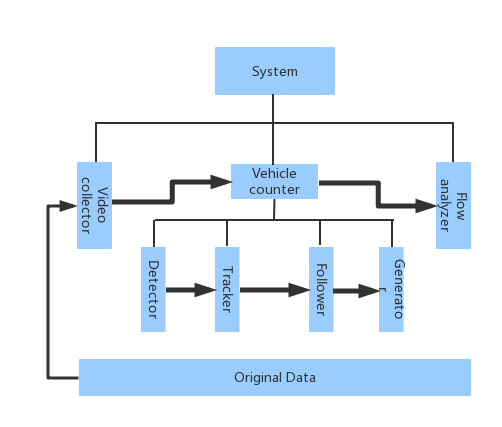
\includegraphics[width=0.4\linewidth]{diagram1.png} 
	\caption{System diagram:Video collector - Vehicle counter - Flow analyzer}
	\label{fig:sysDiagram}
	\end{figure}
	
	
	%============================================================================
	\subsection{Background Subtraction}
	As the monitoring camera is deployed with a fixed position, videos collected from this kind of devices would have a stable background. And the automobile vehicles forms the foreground motions. Hence, content of each frame image contains two parts, foreground and background. To detect the vehicles, we utilize background subtraction method, which can be described as:
	\begin{equation}
	F = I  - B
	\label{eq:backgroundSubtraction}
	\end{equation}
	Where $I$ is derived from frame image, $B$ is the corresponding background, and $F$ is hence the detected foreground.
	
	Frame images from video usually have more than one channel, and they may vary from different types and sizes. This makes it hard or impossible for directing subtraction calculation. Hence, we introduce a collector module to unify the original frame images, as Fig.\ref{fig:unifyDiagram}
	\begin{figure}[!h]
	\centering
%	\subfigure[Original frame image]{
%	\includegraphics[width=0.22\linewidth]{frameImg.jpg}}
	\subfigure[I:image frame]{
	\includegraphics[width=0.32\linewidth]{frameImgGry.jpg}}
	\subfigure[B:background model]{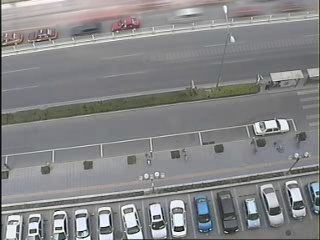
\includegraphics[width=0.32\linewidth]{InitBackgroudFile.jpg}}	
	\subfigure[F:foreground image ]{
	\includegraphics[width=0.32\linewidth]{rawMask.jpg} }
	\caption{Unifying frame image:transform the original image to 8 bits unsigned char with single channel}
	\label{fig:unifyDiagram}
	\end{figure}
	
	After unifying operation, we do background subtraction, and get the foreground image $F$ as Eq.\ref{eq:backgroundSubtraction}. $F$ is mainly consisted of 2 area, the black and the gray. They stands for the background and the foreground separately. However, the gray parts is distributed all the image, making it hard for automobile vehicle detection. Ideally, the gray area of $F$ should gather together as an island. But due to camera performance, environment disturbance and so on, the image carries noise. Even worse,some parts of automobile vehicle may have coincident color with the background overlapping, this would results in gabs and separations.
	\begin{equation}
	  mask=sign(v)=\left\{
	   \begin{aligned}
	   	1, v \geq \delta \\
	   	0, v < \delta \\
	   \end{aligned}
	   \right.
	   \label{eq:foreMask}
	\end{equation}		
	To solve the problem above, we take following strategies as Fig.\ref{fig:preDetection}. First, we employs a Guassian filter with 4*4 size window to reduce noise. Second, we transform the result into binary image with Eq.\ref{eq:foreMask}, the result $Mask$ may consists of several neighbor areas. To make it a nice mask for describing automobile vehicles' shape and position, we employed dilation. Finally, we applied erosion for a better result. 
%	\begin{figure}[!h]
%	\centering
%	\includegraphics[width=0.45\linewidth]{diagram2.png} 
%	\caption{Diagram:Frame image pre-Detection diagram}
%	\label{fig:preDetection}
%	\end{figure}
	
	\begin{figure}[!h]
	\subfigure[Filter Guassian noise]{
	\includegraphics[width=0.22\linewidth]{guassian.jpg} }
	\subfigure[Binary image]{
	\includegraphics[width=0.22\linewidth]{binary.jpg} }
	\subfigure[Dilation]{
	\includegraphics[width=0.22\linewidth]{dilation.jpg} }
	\subfigure[Erosion]{
	\includegraphics[width=0.22\linewidth]{erosion.jpg} }
	\centering
	\caption{Guassian Filter - Binary Image - Dilation - Erosion}
	\label{fig:preDetection}
	\end{figure}




	\subsection{Background Model}
	Frame images consists of two parts, foreground and background. If there were no automobile vehicles within the frame image, the background is hence equal to the frame image. But this is not always the case, as the automobile vehicles are running on the road from time to time. Even worse, background may change due to light, wind and so on. So a steady background model is essential to the robustness of the system.
	Traf first builds the initial background model by averaging first 50 frame images. The result is shown as Fig \ref{fig:backgroundModel}.
%	\begin{figure}[!h]
%	\centering
%	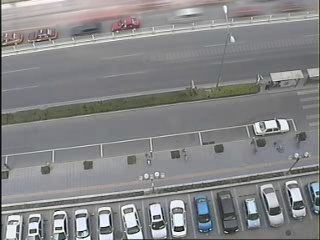
\includegraphics[width=0.4\linewidth]{InitBackgroudFile.jpg} 
%	\caption{Background model construction}
%	\label{fig:backgroundModel}
%	\end{figure}
	 	
	To adapt to environment change, Traf employs an adaptive parameter $\lambda$ as equation \ref{eq:adaption}.
	\begin{equation}
	M_{t} = (1-\lambda)M_{t-1} + \lambda B_{t}
	\label{eq:adaption}
	\end{equation}
	where $M_t$ and $M_{t-1}$ are the background model at time $t$ and $t-1$, $B_{t}$ is the background derived from frame image at time $t$.
	\begin{eqnarray}	
	F_{t}=&I_{t} - M_{t-1}	\\
	B_{t}=&y(F_{t})*M_{t-1}+(1-y(F_{t}))I_{t}
	\end{eqnarray}
Item $B_{t}$ is built from the mask of foreground and background model at time $t$. The mask is derived from a sign function as:
	\begin{equation}
	  y=sign(F)=\left\{
	   \begin{aligned}
	   	1, F \geq \epsilon \\
	   	0, F < \epsilon \\
	   \end{aligned}
	   \right.
	\end{equation}			
	
				
	
	\subsection{Motion}
	After preview operations, $Mask$ becomes a binary image consists of white islands and black background. The white symbolizes vehicle cars within foreground. The following process is to identify these islands, or motion detection. To count the vehicle correctly, we need also to track each detected vehicles.
	
	\subsubsection{Detection}
	We implement detection by detect the contour of the island, then we calculate the area of the island. Considering the size and the shape of a automobile vehicle, it's obviously that islands with small area should be expelled. After the vehicle has been detected, we draw a rectangular box to hold it for further identification and tracking.
	
	
	\subsubsection{Tracking}
	We employ Kalman-filter to tracking the detected car, this is done by building a moving model and estimating position for each frame.	%============================================================================


	%============================================================================
	\subsection{Traffic Flow Analysis}
	
	
	
% compare and check	
\section{Implementation and Evaluation}
	\subsection{Setup}
	\subsection{Methodology}
	\subsection{Result}



\section{Conclusion}


\end{document}